\documentclass{article}

\usepackage{graphicx}
\usepackage{array}
\usepackage[group-separator={,}]{siunitx}
\usepackage{tikz}
\usepackage{hyperref}

%\usepackage{bm}
%\usepackage{graphicx}

\title{Symmetric Three-body Problem Notes}
\author{Scott Hendrickson}

\begin{document}
\maketitle

%%%%%%%%%%%%%%%%%%%%%%%%%%%%%%%%%%%%%%%%
\section{Equations of Motion}

\label{sec:intro}

From Ekeland page 59 (paperback edition):

\begin{quote}
Imagine two stars of equal mass, rotating around their common center of gravity. Newton's law asserts that this is possible, and that the orbit of the two stars will be a circle, along which they travel with equal speed, being exactly opposite to each other at all times. [...] A third body, with very small mass--a comet, for instance--moves along [the axis].
\end{quote}

%%%%%%%%
\begin{figure}[h]
\begin{center}
	%%%%%
	%
	% http://cremeronline.com/LaTeX/minimaltikz.pdf
	%
	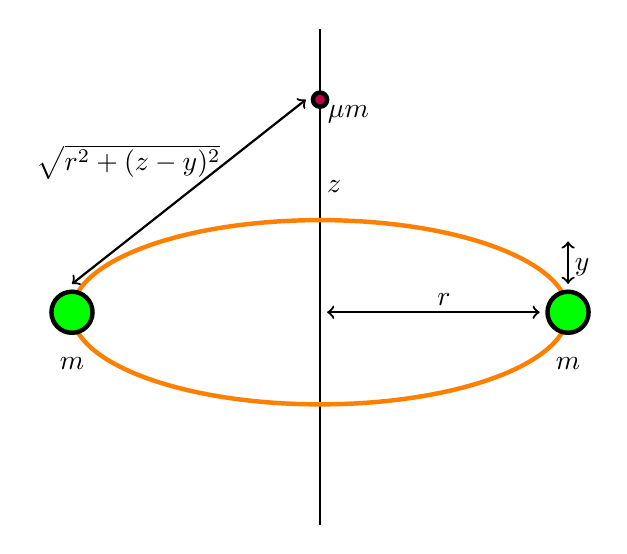
\begin{tikzpicture}[scale=0.9]]
	% arrows
	\draw [thick, -] (0, -3) -- (0,4) ;
	\draw [thick, <->] (0.1, 0) -- (3.1,0) ;
	%\draw [thick, <->] (-0.1, 0) -- (-3.1,0) ;
	\draw [thick, <->] (3.5, 0.4) -- (3.5,1.0) ;
	\draw [thick, <->] (-3.5, 0.4) -- (-0.2,3.0) ;
	% circles
	\draw [orange, ultra thick] (0,0) ellipse (3.5 and 1.3);
	\draw [fill=purple, ultra thick] (0, 3.0) circle [radius=0.1];
	\draw [fill=green, ultra thick] (3.5,0) circle [radius=0.29];
	\draw [fill=green, ultra thick] (-3.5,0) circle [radius=0.29];
	% labels
	\node[align=center, below] at (1.75,0.4){$r$};
	\node[align=center, below] at (3.7,0.9){$y$};
	\node[align=center, below] at (0.2,2){$z$};
	\node[align=center, below] at (3.5,-0.5){$m$};
	\node[align=center, below] at (-3.5,-0.5){$m$};
	\node[align=center, below] at (0.4,3.05){$\mu m$};
	\node[align=center, below] at (-2.7,2.5){$\sqrt{r^2 + (z-y)^2}$};
	\end{tikzpicture}
\end{center}
\caption{Two stars of the same mass $m$ travel in a circular orbit along with a small comet on the centerline with an initial velocity along the z-axis. The system has cylindrical symmetry so that the plain containing the stars moves as a single unit and the comet does not leave the axis. }
\label{fig:tradeoff}
\end{figure}
%%%%%%%%

Gravitational potentials from the interactions of the 3 masses. The first term is the interaction of the
stars while the second term is the sum of the interactions of the comet with each of the stars.

\begin{eqnarray}
U_{m m} & = & \frac{-Gmm}{2r} \\
U_{\mu m} & = & \frac{-2G\mu mm}{\sqrt{r^2 + (z-y)^2}} \\
\label{eq:potentials}
\end{eqnarray}

Kinetic energy terms represent radial, circular and motion along the axis.

\begin{eqnarray}
T & = & \frac{1}{2} \mu m \dot{z}^2 + m \dot{y}^2 + m \dot{r}^2 + m(r\dot{\theta})^2
\label{eq:potentials}
\end{eqnarray}

Lagrangian.

\begin{eqnarray}
\mathcal{L} & = & T - V \\
& = & \frac{1}{2} \mu m \dot{z}^2 + m \dot{y}^2 + m \dot{r}^2 + m(r\dot{\theta})^2 + \frac{-Gmm}{2r} +  \frac{-2G\mu mm}{\sqrt{r^2 + (z-y)^2}}
\label{eq:potentials}
\end{eqnarray}

Partial derivatives with respect to velocities and postitions.

\begin{eqnarray}
\frac{\partial{\mathcal{L}}}{\partial{ \dot{z}}} & = & \mu m \dot{z} \\
\frac{\partial{\mathcal{L}}}{\partial{ \dot{r}}} & = & 2m\dot{r} \\
\frac{\partial{\mathcal{L}}}{\partial{ \dot{y}}} & = & 2m\dot{y} \\
\frac{\partial{\mathcal{L}}}{\partial{ \dot{\theta}}} & = & 2mr^2\dot{\theta} 
\end{eqnarray}

\begin{eqnarray}
\frac{\partial{\mathcal{L}}}{\partial{z}} & = & \frac{2G \mu m^2 (z-y)}{(r^2 + (z-y)^2)^{3/2}} \\
\frac{\partial{\mathcal{L}}}{\partial{r}} & = & 2mr\theta^2 - \frac{G m^2}{r^2} - \frac{2 G \mu m^2 r}{(r^2 + (z-y)^2)^{3/2}} \\
\frac{\partial{\mathcal{L}}}{\partial{y}} & = & - \frac{2G \mu m^2 (z-y)}{(r^2 + (z-y)^2)^{3/2}} \\
\frac{\partial{\mathcal{L}}}{\partial{\theta}} & = & 0 
\end{eqnarray}

Equations of motion,

\begin{eqnarray}
\ddot{z} & = & \frac{2G m (z-y)}{(r^2 + (z-y)^2)^{3/2}} \\
\ddot{y} & = & \frac{G \mu m (z-y)}{(r^2 + (z-y)^2)^{3/2}} \\
\ddot{r} & = & r\dot{\theta}^2 - Gm (\frac{1}{2r^2} + \frac{\mu r}{(r^2 + (z-y)^2)^{3/2}}) \\
\ddot{\theta} & = & \frac{-2 \dot{r} \dot{\theta}}{r} 
\label{eq:mot}
\end{eqnarray}

\noindent can be rewritten as a system of $1^{st}$ differential equations and integrated with a ``Leap frog'' integrator. This
preserves phase space topology.

\begin{figure}[h]
    \begin{center}
        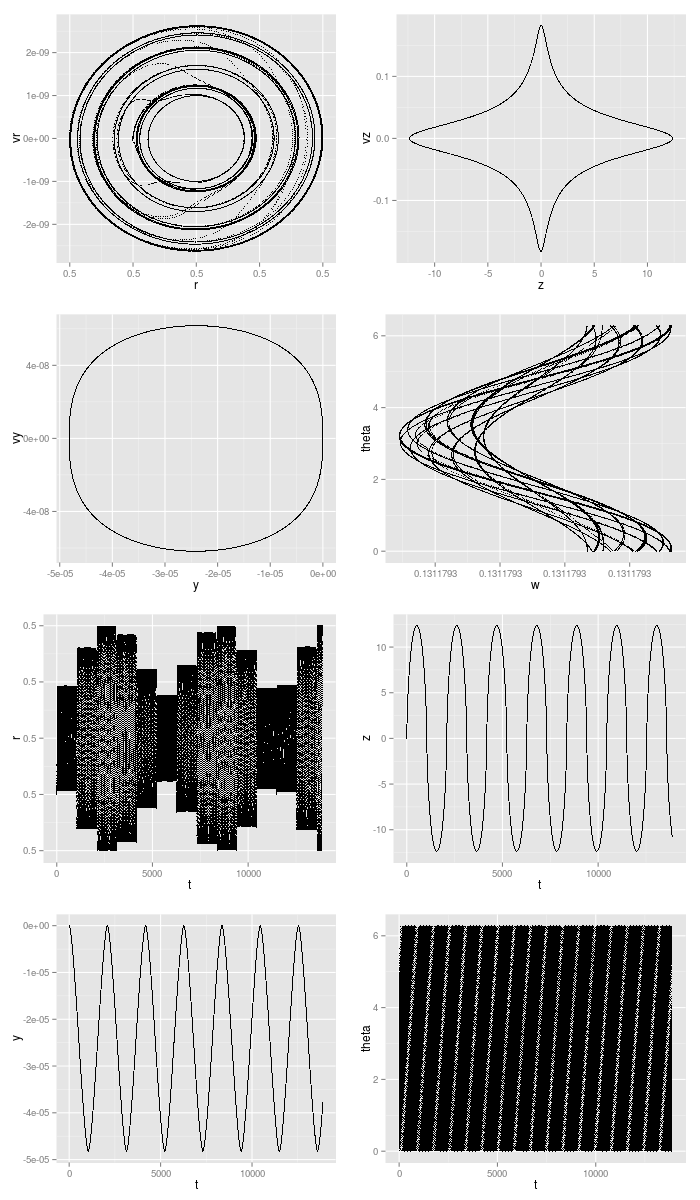
\includegraphics[height=7.75in]{./img/example.png}
    \end{center}
\label{fig:example}
\end{figure}

%
%\begin{table}
%\caption{Fit parameters for Twitter, earthquake.}
%\label{tab:pars}
%\begin{tabular}{ | l | l |}
%    \hline
%    Parameter & Value  \\ \hline
%    $t_0$ & fixxx sec\\ 
%              & 2012-03-20 18:08:22 UTC\\
%    $r_0$ & fixxx act/min\\ 
%    $\alpha$ & 0.001152 sec$^{-1}$\\ 
%    $\beta$ & 0.000220 sec$^{-1}$\\ \hline
%    $t_{time_to_peak}$ & 26 min 30 sec \\ 
%    $S_{vol}$ & 5,568,800 tweets \\
%    $t_{1/2}$ & 92 min 01 sec \\
%    $t_{avg}$ & 87 min 49 sec \\ \hline
%\end{tabular}
%\end{table}
%
%\section{Sigmoid Model}
%\label{sec:sigmodel}
%



%%%%%%%%%%%%%%%%%%%%%%%%%%%%%%%%%%%%%%%%%%%%%%%%%%%%%%%%%%%%%%%%%%%%

\section{Sources and Licensing} 

For code and example output, please visit and fork or clone \url{https://github.com/DrSkippy/Gravitational-Three-Body-Symmetric}.
\noindent If you find errorsor have comments, please email scott@drskippy.net.
\noindent This work is licensed under a Creative Commons CC0 1.0 Universal (CC0 1.0) 
\noindent \url{http://creativecommons.org/publicdomain/zero/1.0/}.

%%%%%%%%%%%%%%%%%%%%%%%%%%%%%%%%%%%%%%%%%%%%%%%%%%%%%%%%%%%%%%%%%%%

\begin{thebibliography}{2013}

\bibitem[Ekeland1990]{Ekeland:1990} Ivar Ekeland. Mathematics and the Unexpected.  \url{http://www.amazon.com/Mathematics-Unexpected-Ivar-Ekeland/dp/0226199908} 1990.

\bibitem[Drexel]{Drexel} The Leapfrog Integrator, \url{http://einstein.drexel.edu/courses/Comp_Phys/Integrators/leapfrog/}.

\end{thebibliography}

\end{document}
